\documentclass[border=4pt]{standalone}
\usepackage{tikz}
\usetikzlibrary{
  positioning, arrows.meta, calc, backgrounds,
  decorations.pathreplacing, fit
}
\usepackage{amsmath}

\begin{document}
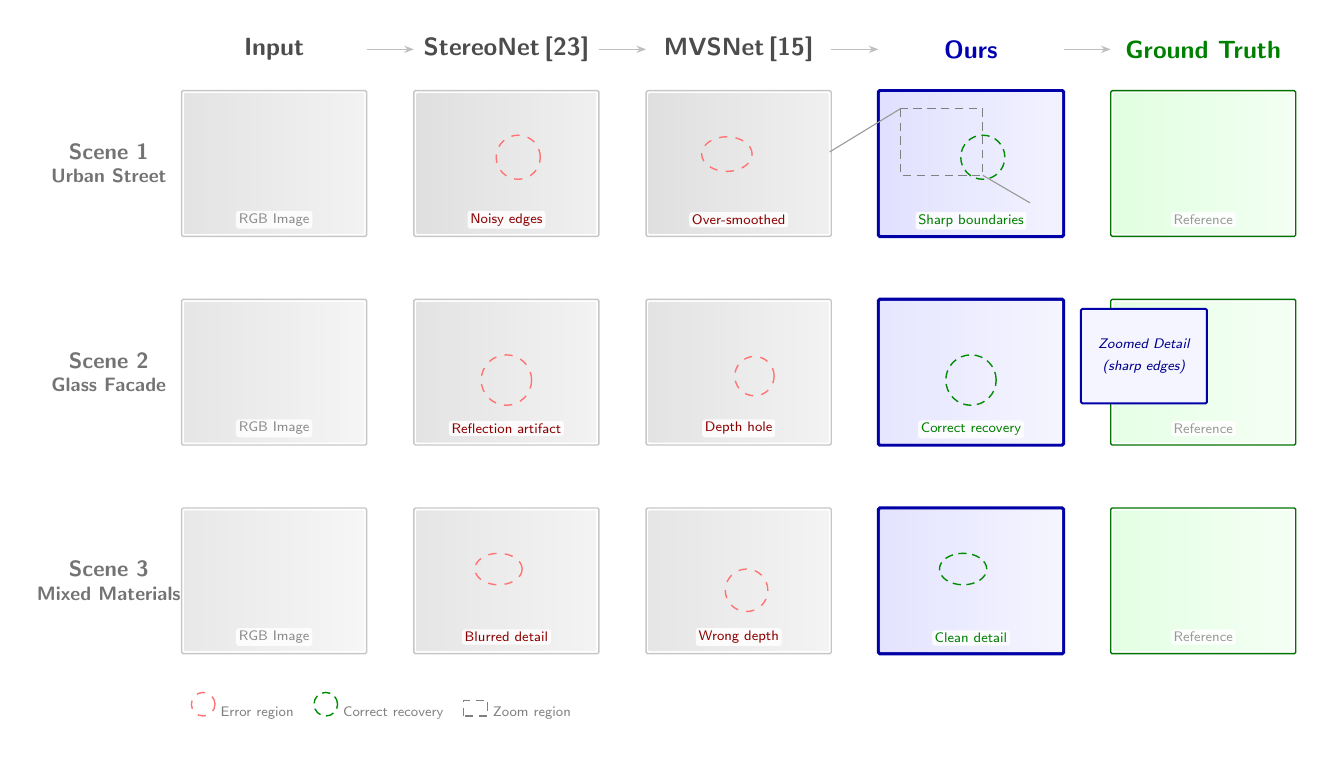
\begin{tikzpicture}[
  imgbox/.style={
    draw=gray!45, minimum width=2.35cm, minimum height=1.85cm,
    inner sep=0pt, line width=0.5pt, rounded corners=0.5pt
  },
  ourbox/.style={
    draw=blue!65!black, minimum width=2.35cm, minimum height=1.85cm,
    inner sep=0pt, line width=1.2pt, rounded corners=0.5pt
  },
  gtbox/.style={
    draw=green!45!black, minimum width=2.35cm, minimum height=1.85cm,
    inner sep=0pt, line width=0.5pt, rounded corners=0.5pt
  },
  colhdr/.style={font=\sffamily\small\bfseries, text=black!70},
  rowlbl/.style={font=\sffamily\footnotesize\bfseries, text=black!55, align=center},
  sublbl/.style={font=\sffamily\tiny, text=#1, fill=white, fill opacity=0.85,
                 text opacity=1, inner sep=1pt, rounded corners=1pt},
  sublbl/.default={black!45},
  flowarr/.style={-{Stealth[length=3.5pt]}, color=black!25, line width=0.6pt},
  errcirc/.style={draw=red!55, dashed, line width=0.5pt},
  goodcirc/.style={draw=green!55!black, densely dashed, line width=0.5pt},
]

% --- Column positions (center x) ---
\def\colA{0}
\def\colB{2.95}
\def\colC{5.9}
\def\colD{8.85}
\def\colE{11.8}

% --- Row positions (center y) ---
\def\rowA{0}
\def\rowB{-2.65}
\def\rowC{-5.3}

% --- Column Headers ---
\node[colhdr] at (\colA, 1.45) {Input};
\node[colhdr] at (\colB, 1.45) {StereoNet\,[23]};
\node[colhdr] at (\colC, 1.45) {MVSNet\,[15]};
\node[colhdr, text=blue!70!black] at (\colD, 1.45) {Ours};
\node[colhdr, text=green!50!black] at (\colE, 1.45) {Ground Truth};

% --- Flow arrows between headers ---
\draw[flowarr] ($( \colA+1.175, 1.45)$) -- ($( \colB-1.175, 1.45)$);
\draw[flowarr] ($( \colB+1.175, 1.45)$) -- ($( \colC-1.175, 1.45)$);
\draw[flowarr] ($( \colC+1.175, 1.45)$) -- ($( \colD-1.175, 1.45)$);
\draw[flowarr] ($( \colD+1.175, 1.45)$) -- ($( \colE-1.175, 1.45)$);

% --- Scene Labels (left side) ---
\node[rowlbl] at (-2.1, \rowA) {Scene 1\\[-1pt]{\scriptsize Urban Street}};
\node[rowlbl] at (-2.1, \rowB) {Scene 2\\[-1pt]{\scriptsize Glass Facade}};
\node[rowlbl] at (-2.1, \rowC) {Scene 3\\[-1pt]{\scriptsize Mixed Materials}};

% ======================================================================
% ROW 1 — Urban Street
% ======================================================================
\node[imgbox] (r1c1) at (\colA, \rowA) {};
\shade[left color=gray!22, right color=gray!10, rounded corners=0.3pt]
  ($(r1c1.north west)+(0.04,-0.04)$) rectangle ($(r1c1.south east)+(-0.04,0.04)$);
\node[sublbl] at ($(r1c1.south)+(0,0.22)$) {RGB Image};

\node[imgbox] (r1c2) at (\colB, \rowA) {};
\shade[left color=gray!25, right color=gray!12, rounded corners=0.3pt]
  ($(r1c2.north west)+(0.04,-0.04)$) rectangle ($(r1c2.south east)+(-0.04,0.04)$);
\draw[errcirc] ($(r1c2.center)+(0.15,0.08)$) circle (0.28cm);
\node[sublbl={red!55!black}] at ($(r1c2.south)+(0,0.22)$) {Noisy edges};

\node[imgbox] (r1c3) at (\colC, \rowA) {};
\shade[left color=gray!25, right color=gray!12, rounded corners=0.3pt]
  ($(r1c3.north west)+(0.04,-0.04)$) rectangle ($(r1c3.south east)+(-0.04,0.04)$);
\draw[errcirc] ($(r1c3.center)+(-0.15,0.12)$) ellipse (0.32cm and 0.22cm);
\node[sublbl={red!55!black}] at ($(r1c3.south)+(0,0.22)$) {Over-smoothed};

\node[ourbox] (r1c4) at (\colD, \rowA) {};
\shade[left color=blue!12, right color=blue!5, rounded corners=0.3pt]
  ($(r1c4.north west)+(0.04,-0.04)$) rectangle ($(r1c4.south east)+(-0.04,0.04)$);
\draw[goodcirc] ($(r1c4.center)+(0.15,0.08)$) circle (0.28cm);
\node[sublbl={green!50!black}] at ($(r1c4.south)+(0,0.22)$) {Sharp boundaries};

\node[gtbox] (r1c5) at (\colE, \rowA) {};
\shade[left color=green!12, right color=green!5, rounded corners=0.3pt]
  ($(r1c5.north west)+(0.04,-0.04)$) rectangle ($(r1c5.south east)+(-0.04,0.04)$);
\node[sublbl={black!40}] at ($(r1c5.south)+(0,0.22)$) {Reference};

% ======================================================================
% ROW 2 — Glass Facade
% ======================================================================
\node[imgbox] (r2c1) at (\colA, \rowB) {};
\shade[left color=gray!20, right color=gray!8, rounded corners=0.3pt]
  ($(r2c1.north west)+(0.04,-0.04)$) rectangle ($(r2c1.south east)+(-0.04,0.04)$);
\node[sublbl] at ($(r2c1.south)+(0,0.22)$) {RGB Image};

\node[imgbox] (r2c2) at (\colB, \rowB) {};
\shade[left color=gray!22, right color=gray!10, rounded corners=0.3pt]
  ($(r2c2.north west)+(0.04,-0.04)$) rectangle ($(r2c2.south east)+(-0.04,0.04)$);
\draw[errcirc] ($(r2c2.center)+(0.0,-0.1)$) circle (0.32cm);
\node[sublbl={red!55!black}] at ($(r2c2.south)+(0,0.22)$) {Reflection artifact};

\node[imgbox] (r2c3) at (\colC, \rowB) {};
\shade[left color=gray!22, right color=gray!10, rounded corners=0.3pt]
  ($(r2c3.north west)+(0.04,-0.04)$) rectangle ($(r2c3.south east)+(-0.04,0.04)$);
\draw[errcirc] ($(r2c3.center)+(0.2,-0.05)$) circle (0.25cm);
\node[sublbl={red!55!black}] at ($(r2c3.south)+(0,0.22)$) {Depth hole};

\node[ourbox] (r2c4) at (\colD, \rowB) {};
\shade[left color=blue!10, right color=blue!4, rounded corners=0.3pt]
  ($(r2c4.north west)+(0.04,-0.04)$) rectangle ($(r2c4.south east)+(-0.04,0.04)$);
\draw[goodcirc] ($(r2c4.center)+(0.0,-0.1)$) circle (0.32cm);
\node[sublbl={green!50!black}] at ($(r2c4.south)+(0,0.22)$) {Correct recovery};

\node[gtbox] (r2c5) at (\colE, \rowB) {};
\shade[left color=green!10, right color=green!4, rounded corners=0.3pt]
  ($(r2c5.north west)+(0.04,-0.04)$) rectangle ($(r2c5.south east)+(-0.04,0.04)$);
\node[sublbl={black!40}] at ($(r2c5.south)+(0,0.22)$) {Reference};

% ======================================================================
% ROW 3 — Mixed Materials
% ======================================================================
\node[imgbox] (r3c1) at (\colA, \rowC) {};
\shade[left color=gray!18, right color=gray!7, rounded corners=0.3pt]
  ($(r3c1.north west)+(0.04,-0.04)$) rectangle ($(r3c1.south east)+(-0.04,0.04)$);
\node[sublbl] at ($(r3c1.south)+(0,0.22)$) {RGB Image};

\node[imgbox] (r3c2) at (\colB, \rowC) {};
\shade[left color=gray!20, right color=gray!9, rounded corners=0.3pt]
  ($(r3c2.north west)+(0.04,-0.04)$) rectangle ($(r3c2.south east)+(-0.04,0.04)$);
\draw[errcirc] ($(r3c2.center)+(-0.1,0.15)$) ellipse (0.3cm and 0.2cm);
\node[sublbl={red!55!black}] at ($(r3c2.south)+(0,0.22)$) {Blurred detail};

\node[imgbox] (r3c3) at (\colC, \rowC) {};
\shade[left color=gray!20, right color=gray!9, rounded corners=0.3pt]
  ($(r3c3.north west)+(0.04,-0.04)$) rectangle ($(r3c3.south east)+(-0.04,0.04)$);
\draw[errcirc] ($(r3c3.center)+(0.1,-0.12)$) circle (0.27cm);
\node[sublbl={red!55!black}] at ($(r3c3.south)+(0,0.22)$) {Wrong depth};

\node[ourbox] (r3c4) at (\colD, \rowC) {};
\shade[left color=blue!11, right color=blue!4, rounded corners=0.3pt]
  ($(r3c4.north west)+(0.04,-0.04)$) rectangle ($(r3c4.south east)+(-0.04,0.04)$);
\draw[goodcirc] ($(r3c4.center)+(-0.1,0.15)$) ellipse (0.3cm and 0.2cm);
\node[sublbl={green!50!black}] at ($(r3c4.south)+(0,0.22)$) {Clean detail};

\node[gtbox] (r3c5) at (\colE, \rowC) {};
\shade[left color=green!11, right color=green!4, rounded corners=0.3pt]
  ($(r3c5.north west)+(0.04,-0.04)$) rectangle ($(r3c5.south east)+(-0.04,0.04)$);
\node[sublbl={black!40}] at ($(r3c5.south)+(0,0.22)$) {Reference};

% ======================================================================
% Zoom-in detail box for Ours (Row 1)
% ======================================================================
\draw[black!50, line width=0.5pt, densely dashed]
  ($(r1c4.north west)+(0.3,-0.25)$) rectangle ($(r1c4.center)+(0.15,-0.15)$);
\draw[black!40, line width=0.4pt]
  ($(r1c4.center)+(0.15,-0.15)$) -- ++(0.6,-0.35)
  ($(r1c4.north west)+(0.3,-0.25)$) -- ++(-0.9,-0.55);

% Zoom inset box
\node[draw=blue!65!black, line width=0.7pt, fill=blue!4, rounded corners=0.5pt,
      minimum width=1.6cm, minimum height=1.2cm, inner sep=0pt,
      font=\sffamily\tiny\itshape, text=blue!55!black, align=center]
  (zoom1) at ($(r1c4.south east)+(1.0,-1.5)$) {Zoomed Detail\\[2pt](sharp edges)};

% ======================================================================
% Legend at the bottom
% ======================================================================
\node[anchor=north west, font=\sffamily\tiny, text=black!50, align=left]
  at ($(r3c1.south west)+(0,-0.35)$)
  {\tikz\draw[errcirc] (0,0) circle (0.15cm); Error region \quad
   \tikz\draw[goodcirc] (0,0) circle (0.15cm); Correct recovery \quad
   \tikz\draw[black!50, line width=0.5pt, densely dashed] (0,0) rectangle (0.3,0.2); Zoom region};

\end{tikzpicture}
\end{document}